\documentclass{article}
\usepackage[utf8]{inputenc}
\usepackage{fullpage}
\usepackage{graphicx}
\usepackage{listings}
\usepackage{color}
\definecolor{codegreen}{rgb}{0,0.6,0}
\definecolor{codegray}{rgb}{0.5,0.5,0.5}
\definecolor{codepurple}{rgb}{0.58,0,0.82}
\definecolor{backcolour}{rgb}{0.95,0.95,0.92}
\definecolor{codeorange}{RGB}{255,127,80}
 
\lstdefinestyle{mystyle}{
    backgroundcolor=\color{backcolour},   
    commentstyle=\color{codegreen},
    keywordstyle=\color{codeorange},
    numberstyle=\tiny\color{codegray},
    stringstyle=\color{codepurple},
    basicstyle=\footnotesize,
    breakatwhitespace=false,         
    breaklines=true,                 
    captionpos=b,                    
    keepspaces=true,                 
    numbers=left,                    
    numbersep=5pt,                  
    showspaces=false,                
    showstringspaces=false,
    showtabs=false,                  
    tabsize=2
}
\lstset{style=mystyle}


\title{CS112 Final Project: \\ Predicting Civil Conflicts}
\author{Zitong Mao \\ Minerva Schools at KGI}

\begin{document}

\maketitle

\section{Abstract}
Civil wars are increasingly prevalent and lethal, providing an important threat to human security. Various studies have been done to research the relationship between social factors and the onsets of civil conflicts. However, as pointed out by Ward et al. (2010), "too little attention has been paid to finding variables that improve our ability to predict civil wars." Achieving statistically significant results does not necessarily increase the predictive power of existing models. In this paper, I will start with a replication of Ward et al.'s findings. Then, focusing on Ward et al.'s problem of using the original data set as both the training and test set, I will implement a k-fold Cross Validation to predict out-of-sample results. Finally, I will construct a Recursive Partitioning and Regression Trees (RPART) model and a Random Forest model to increase the predictive power of the models without changing the independent variables. I will end the paper with discussions as a decision memo for current researchers.

\section{Replication: Ward et al., 2010}

Ward et al. used Fearon \& Laitin's (2003) data and model to investigate the relative importance of different predictors on the onsets of civil wars. Table \ref{variable} shows the variables used in FL's model\footnote{\#replication}.

\begin{table}[h!]
\centering
\caption{Independent Variables in Fearon \& Laitin's Model}
\label{variable}
\begin{tabular}{lc}
\hline
\textit{Variables}                    & \textit{Statistically significant at 0.05 level} \\ \hline
Prior War (\textbf{warl})                      & Yes                                              \\
GDP per capita (\textbf{gdpenl})               & Yes                                              \\
Population (\textbf{lpopl1})                   & Yes                                              \\
Mountainous Terrain (\textbf{lmtnest})         & Yes                                              \\
Non-contiguous State (\textbf{ncontig})        & No                                               \\
Oil Exporter (\textbf{Oil})                    & Yes                                              \\
New State (\textbf{nwstate})                   & Yes                                              \\
Instability (\textbf{instab})                  & Yes                                              \\
Democracy (\textbf{polity2l})                  & No                                               \\
Ethnic Fractionalization (\textbf{ethfrac})    & No                                               \\
Religious Fractionalization (\textbf{relfrac}) & No                                              
\end{tabular}
\end{table}

With all these eleven predictors, Ward et al. made a logistic regression (Listing 1) to predict the probability of civil wars in different locations. In addition, they created a ROC Plot (Figure \ref{roc1}) and calculated the Area Under Curve to show the predictive power of this model. 



\begin{lstlisting}[language=R, caption=FL Original Model - Logistic Regression]
flmodel <- glm(as.factor(onset) ~ 
                 warl + gdpenl + lpopl1 + lmtnest + ncontig + 
                 Oil + nwstate + instab + polity2l
               + ethfrac + relfrac, family = binomial(link = logit),
               data = fl.three) #no out-of-sample prediction
phat<-predict.glm(flmodel,type="response")
\end{lstlisting}

\begin{figure}[h!]
    \centering
    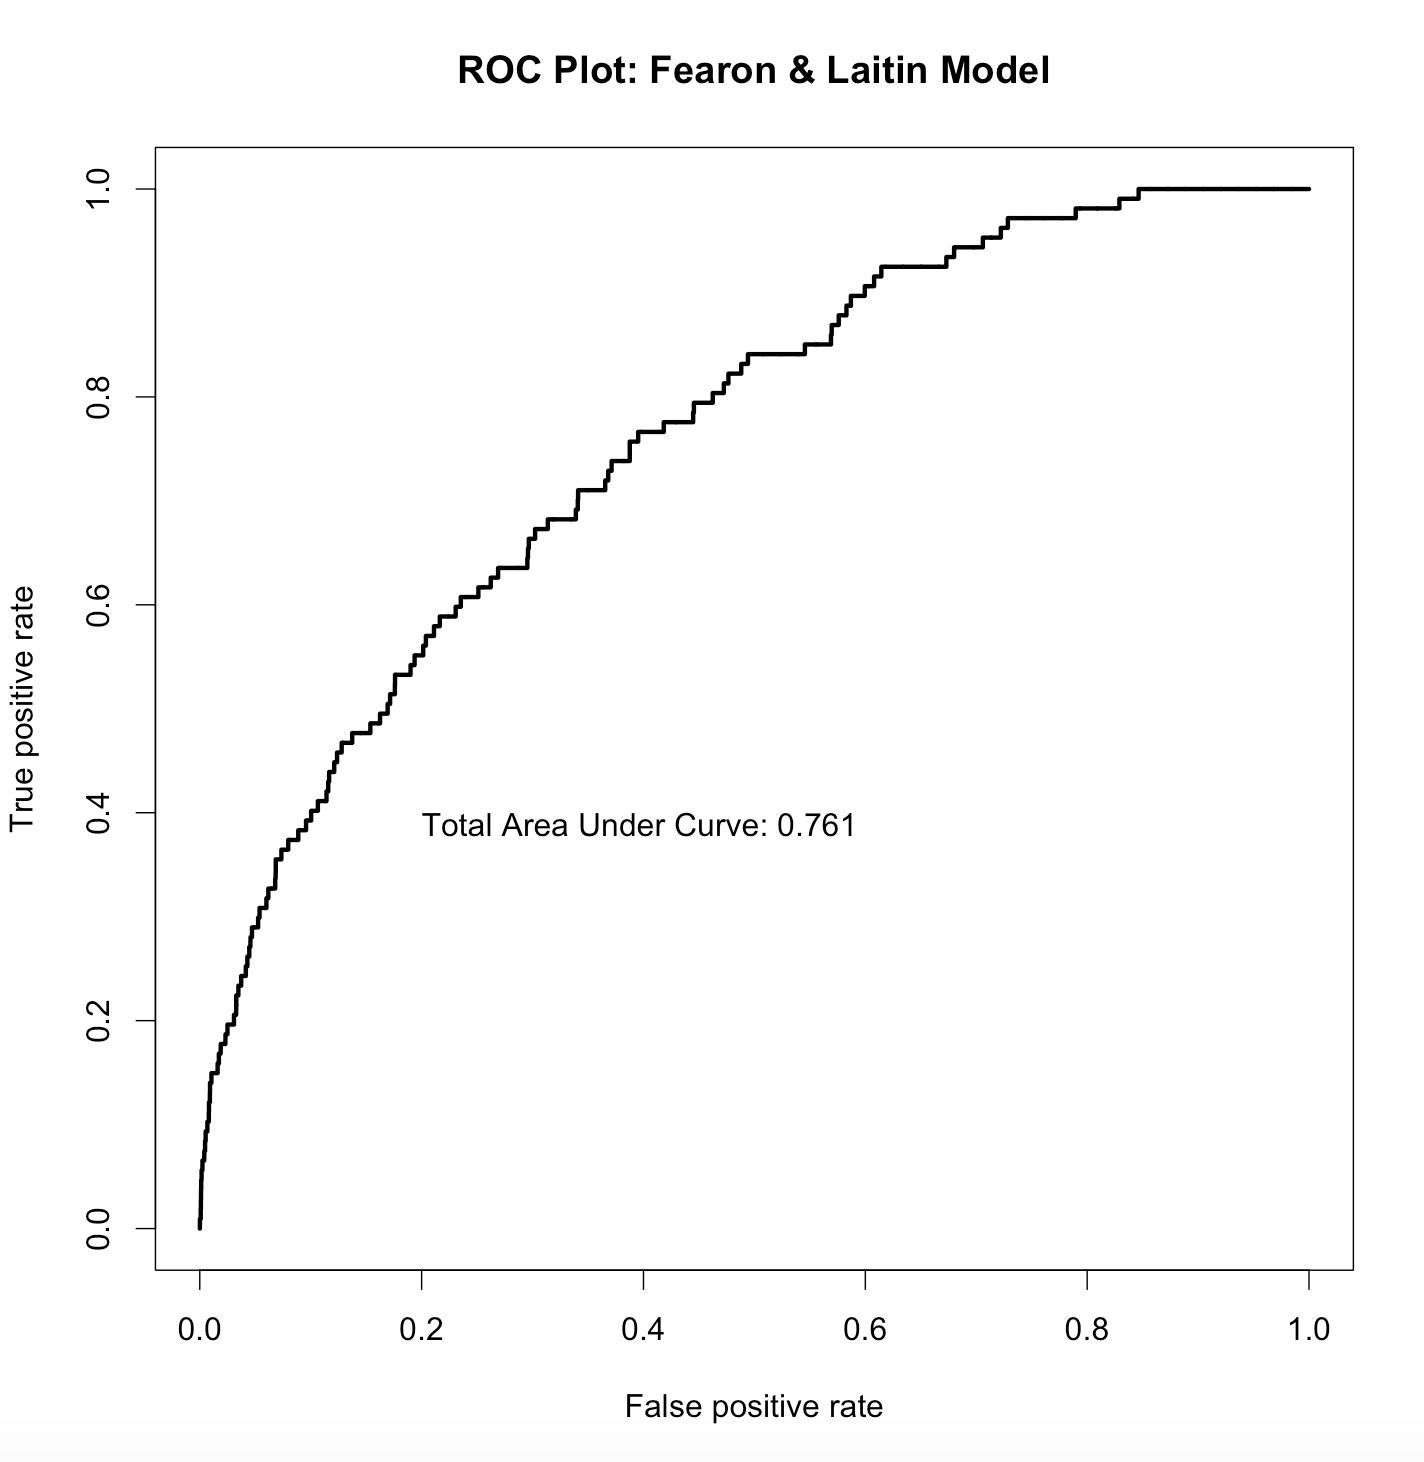
\includegraphics[width=0.5\linewidth]{roc1.png}
    \caption{ROC Plot: Fearon \& Laitin Model}
    \label{roc1}
\end{figure}

I agree with Ward et al.'s conclusion that current models lack the predictive power, and finding statistically significant predictors should not be the only focus for researchers. However, I find their approach to this conclusion somehow problematic. 

\section{Problems}

As we can see in Listing 1, Ward et al. constructed the regression model based on the original dataset with no specification of the training set or the test set. As a result, the ROC Plot only reflects the in-sample predictions. This is a huge problem. Since the topic of this research is "predicting civil conflicts," models with no specifications of training set and test set are not useful at all. Only the \textbf{out-of-sample} results could show us the actual predictive power of the models. Civil wars happening in the future would not be in your old dataset yet. If the models have succeeded in capturing the underlying relationship between the independent and dependent variables, they should still be able to predict events that they have not seen in the training set before.\footnote{\#sampling}\footnote{\#plausibility}

Another problem is that Ward et al. only used the logistic regression model for predicting civil wars. Logistic regression models, especially getting trained only by the full dataset, can suffer from the problem of over-fitting. Their ability to make correct predictions in a new dataset will turn out to be much poorer.\footnote{\#critique}

The main difficulty for conducting out-of-sample research on civil conflicts is that the number of civil wars is limited. There is not any civil conflict that has not been examined before. Therefore, it is extremely difficult to find new data to test existing models.

One possible solution is to perform a \textbf{Cross Validation} to separate existing data set into two parts, training set and test set. After the Cross Validation, the models will be trained only with training set, and their performances will be tested with test set. This allows us to get an overall estimation of the out-of-sample predictive power of a given model without having to find new data.\footnote{\#constraints}

\section{k-fold Cross Validation}

Although various packages in R have built-in Cross Validation functions, I still wrote my original version of k-fold Cross Validation in order to compare the performances of multiple models at the same time with the same Cross Validation Method. Please see the \textit{Appendix} for the full code. It is highly readable, and the k can be easily changed to any other numbers\footnote{\#presentation}.

\begin{lstlisting}[language=R, caption=Logistic Regression Model (Cross-Validated)]
# k-fold cross validation method
k = 5 # Folds

# sample from 1 to k, nrow times (the number of observations in the data_test)
data_test$id <- sample(1:k, nrow(data_test), replace = TRUE)
list <- 1:k

# prediction and testset data_test frames that we add to with each iteration over
# the folds
prediction.f <- data.frame()
prediction <- data.frame()
testsetCopy <- data.frame()

# creating a progress bar to visualize the CV process
progress.bar <- create_progress_bar("text")
progress.bar$init(k)

# loop for k times
for (i in 1:k) {
  # remove rows with id i from data_testframe to create training set
  # select rows with id i to create test set
  trainingset <- subset(data_test, id %in% list[-i]) #[-i] means except i
  testset <- subset(data_test, id %in% list[i])
 
  # run the logistic regression model using training set
  flmodel <- glm(as.factor(onset) ~ 
                    warl + gdpenl + lpopl1 + lmtnest + ncontig + 
                    Oil + nwstate + instab + polity2l
                   + ethfrac + relfrac, family = binomial(link = logit),
                   data = trainingset)
  
  # getting predicted results
  temp <- as.data.frame(predict.glm(flmodel, testset, type="response"))
  temp.f <- ifelse(temp > 0.3, 1, 0) # threshold
  
  # append this iteration's predictions to the end of the prediction data_test frame
  prediction <- rbind(prediction, temp)
  prediction.f <- rbind(prediction.f, temp.f)
  
  # append this iteration's test set to the test set copy data frame
  testsetCopy <- rbind(testsetCopy, as.data.frame(testset))
  
  progress.bar$step()
}

# add predictions and actual dependent variables values
result <- cbind(prediction.f, testsetCopy$onset)
names(result) <- c("Predicted", "Actual")
\end{lstlisting}

The performance of the original Logistic Regression Model dropped from 0.761 to 0.741 after I performed the 5-fold Cross Validation. See Figure \ref{roclr} for the new ROC Plot.

\begin{figure}[h!]
    \centering
    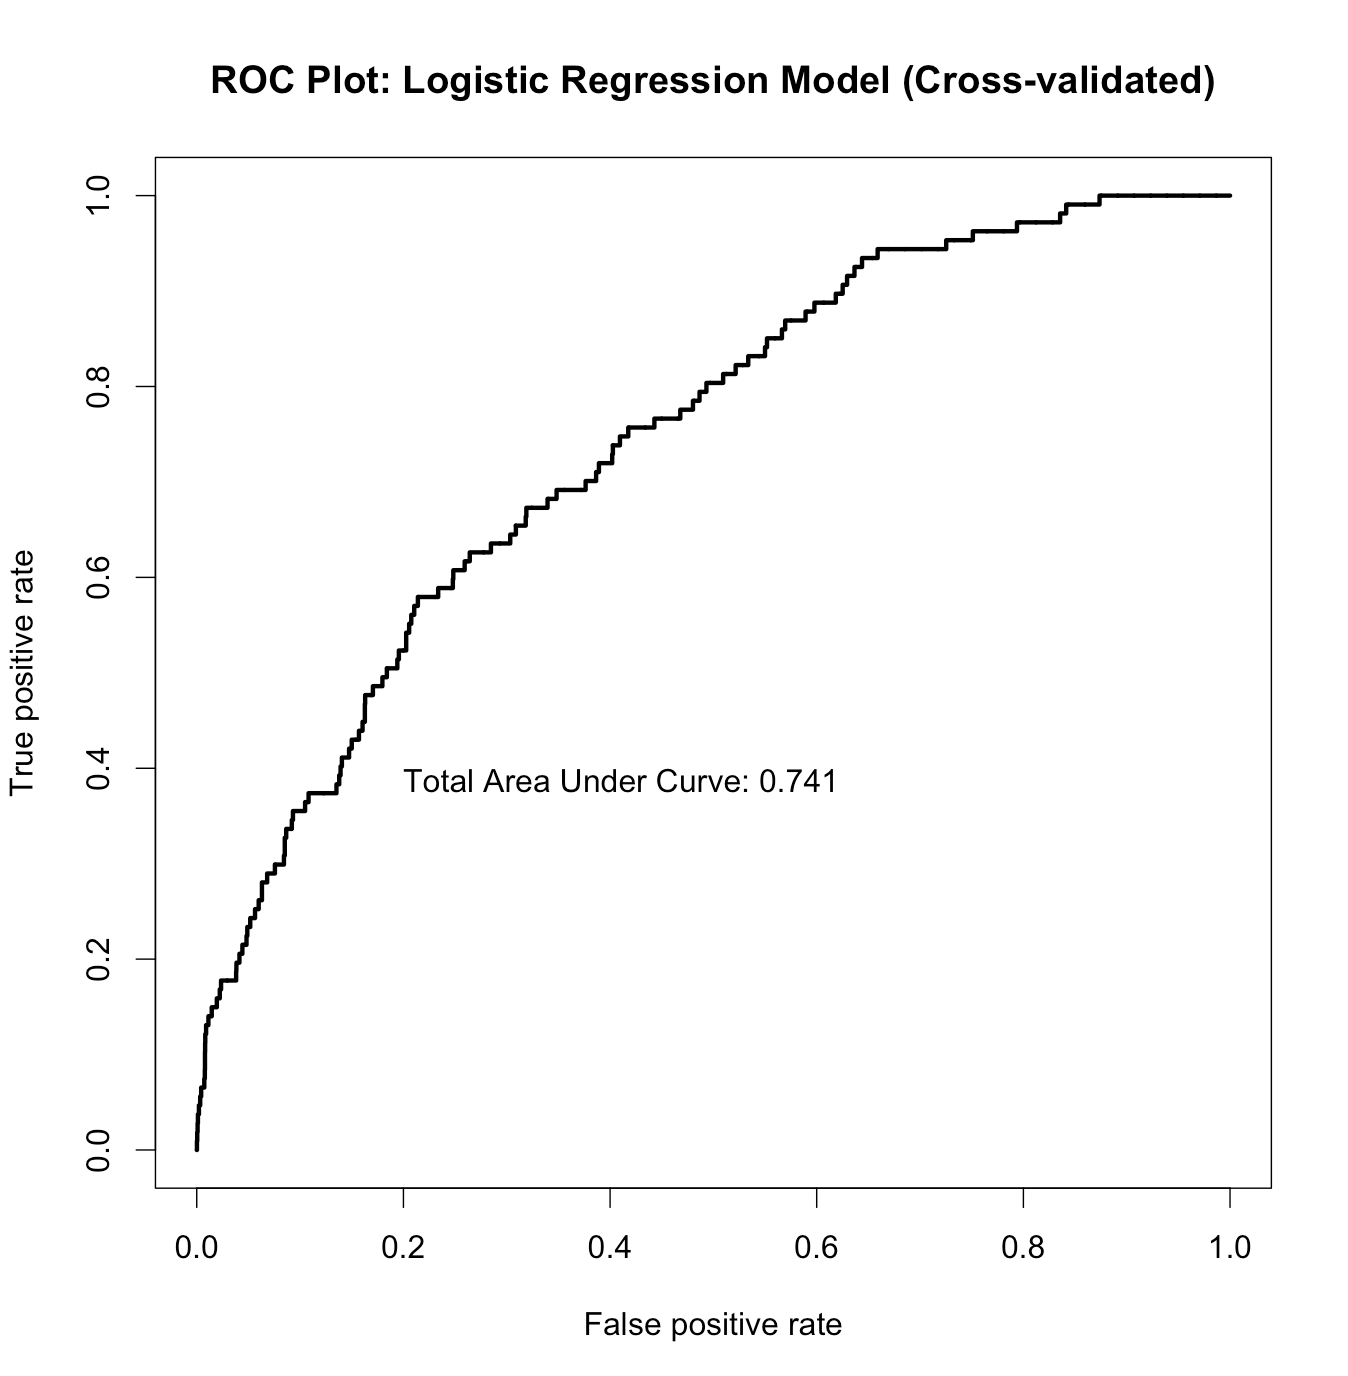
\includegraphics[width=0.5\linewidth]{roclr.png}
    \caption{ROC Plot: Logistic Regression Model (Cross-validated)}
    \label{roclr}
\end{figure}


\section{RPART - Recursive Partitioning and Regression Trees}
I implemented a RPART model (Listing 3) to solve the potential overfitting issues of the regression model to increase the predictive power.\footnote{\#decisiontrees}

\begin{lstlisting}[language=R, caption=RPART Model (Cross-Validated)]
flmodel.rpart <- rpart(as.factor(onset) ~ 
                         warl + gdpenl + lpopl1 + lmtnest + ncontig + 
                         Oil + nwstate + instab + polity2l
                       + ethfrac + relfrac, data = trainingset, 
                       control=rpart.control(minsplit=6, minbucket=2, cp=0.003)) #loosing the control for better predictive power
\end{lstlisting}

The performance increased from 0.741 to 0.756.\footnote{\#prediction} See Figure \ref{rocrpart} for the ROC Plot and Figure \ref{rpart} for a plot of this method.

\begin{figure}[h!]
    \centering
    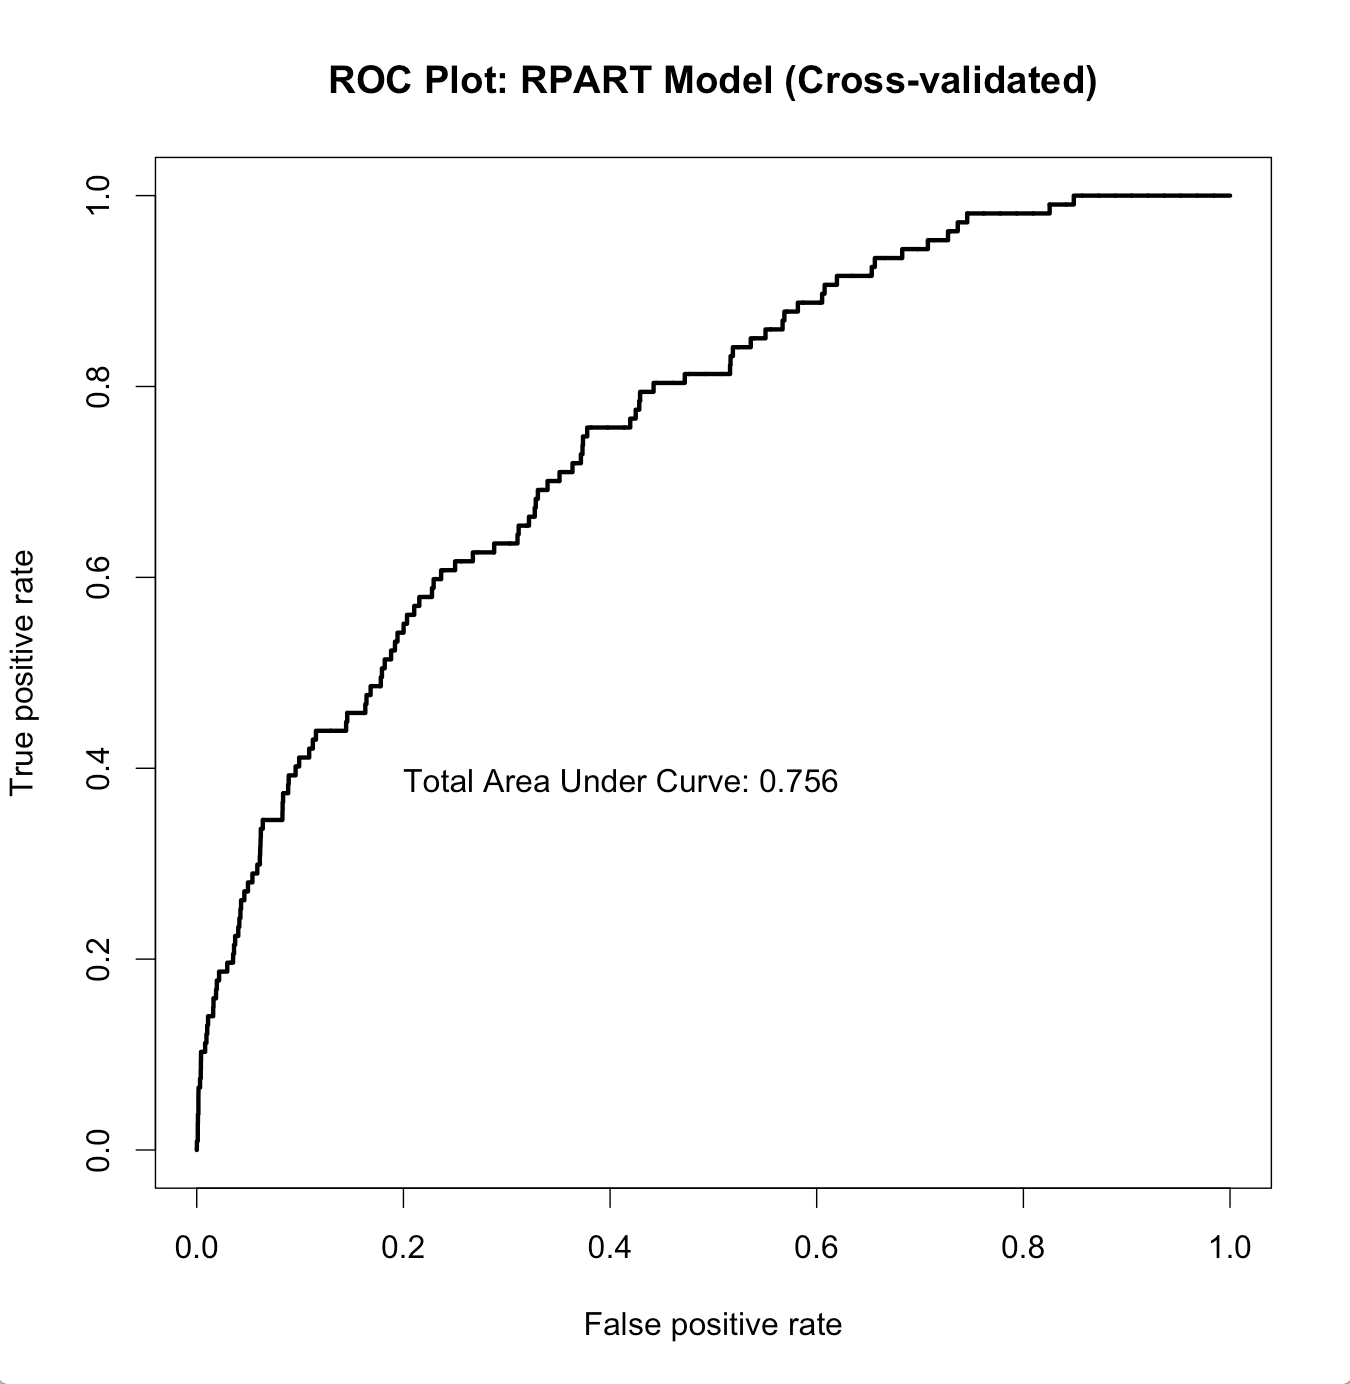
\includegraphics[width=0.5\linewidth]{rocrpart.png}
    \caption{ROC Plot: RPART Model (Cross-validated)}
    \label{rocrpart}
\end{figure}

\begin{figure}[h]
    \centering
    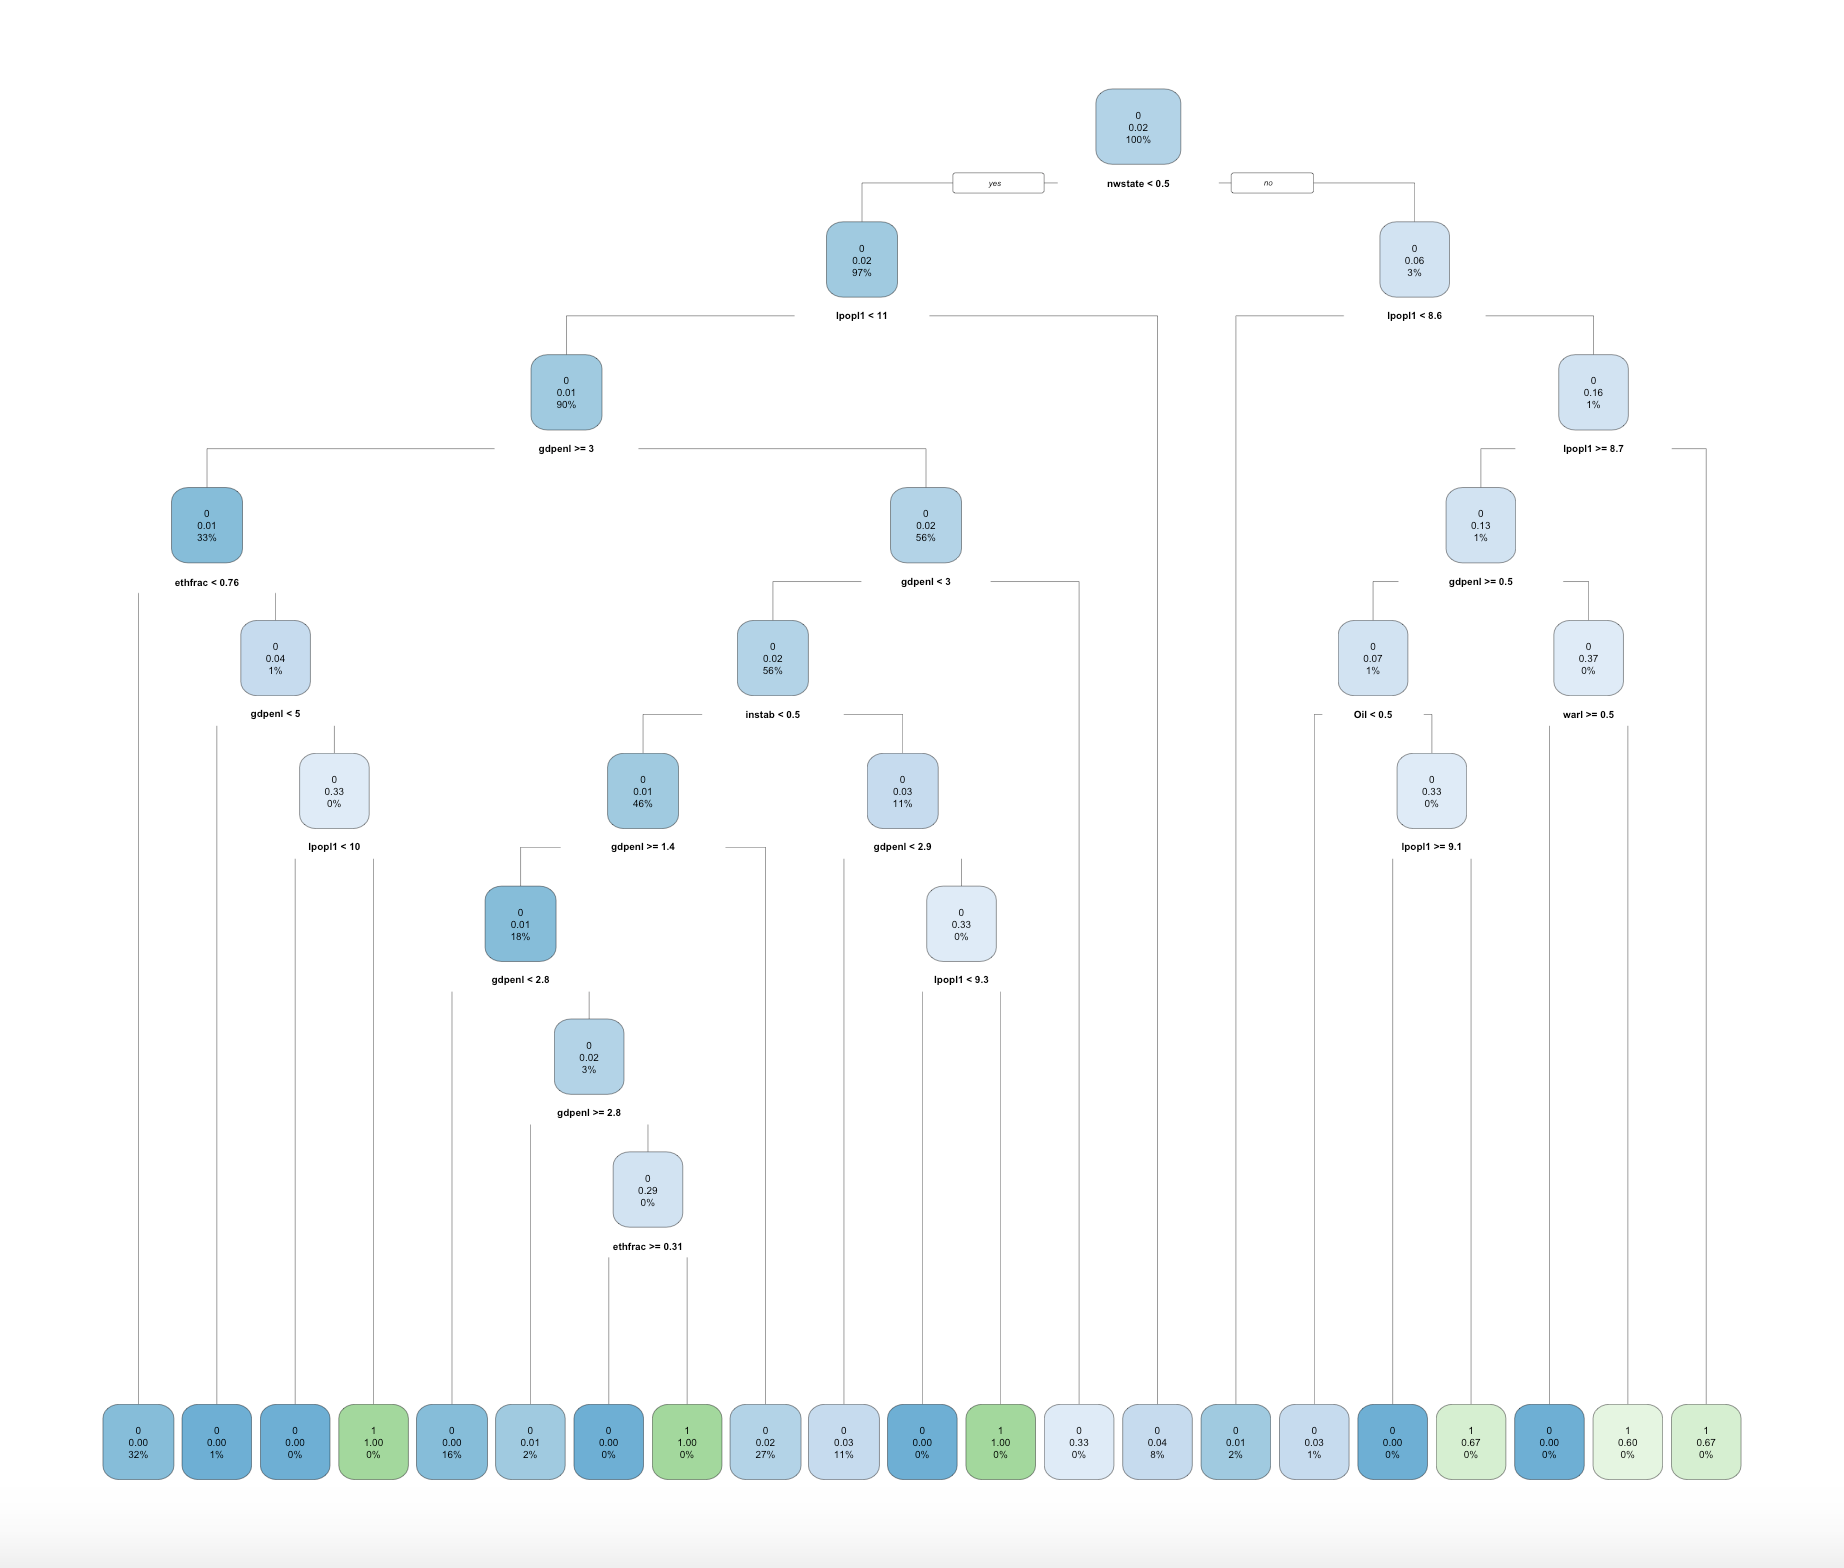
\includegraphics[width=\linewidth]{rpart.png}
    \caption{RPART Plot}
    \label{rpart}
\end{figure}

\section{Random Forest}
I implemented a Random Forest model (Listing 4) in the hope of increasing the performance of the current RPART model.
\begin{lstlisting}[language=R, caption=Random Forest Model (Cross-Validated)]
flmodel.forest <- randomForest(onset ~ warl + gdpenl + 
                                 lpopl1 + lmtnest + ncontig + 
                                 Oil + nwstate + instab + polity2l
                               + ethfrac + relfrac, data = trainingset, importance = TRUE)
\end{lstlisting}

\begin{figure}[h!]
    \centering
    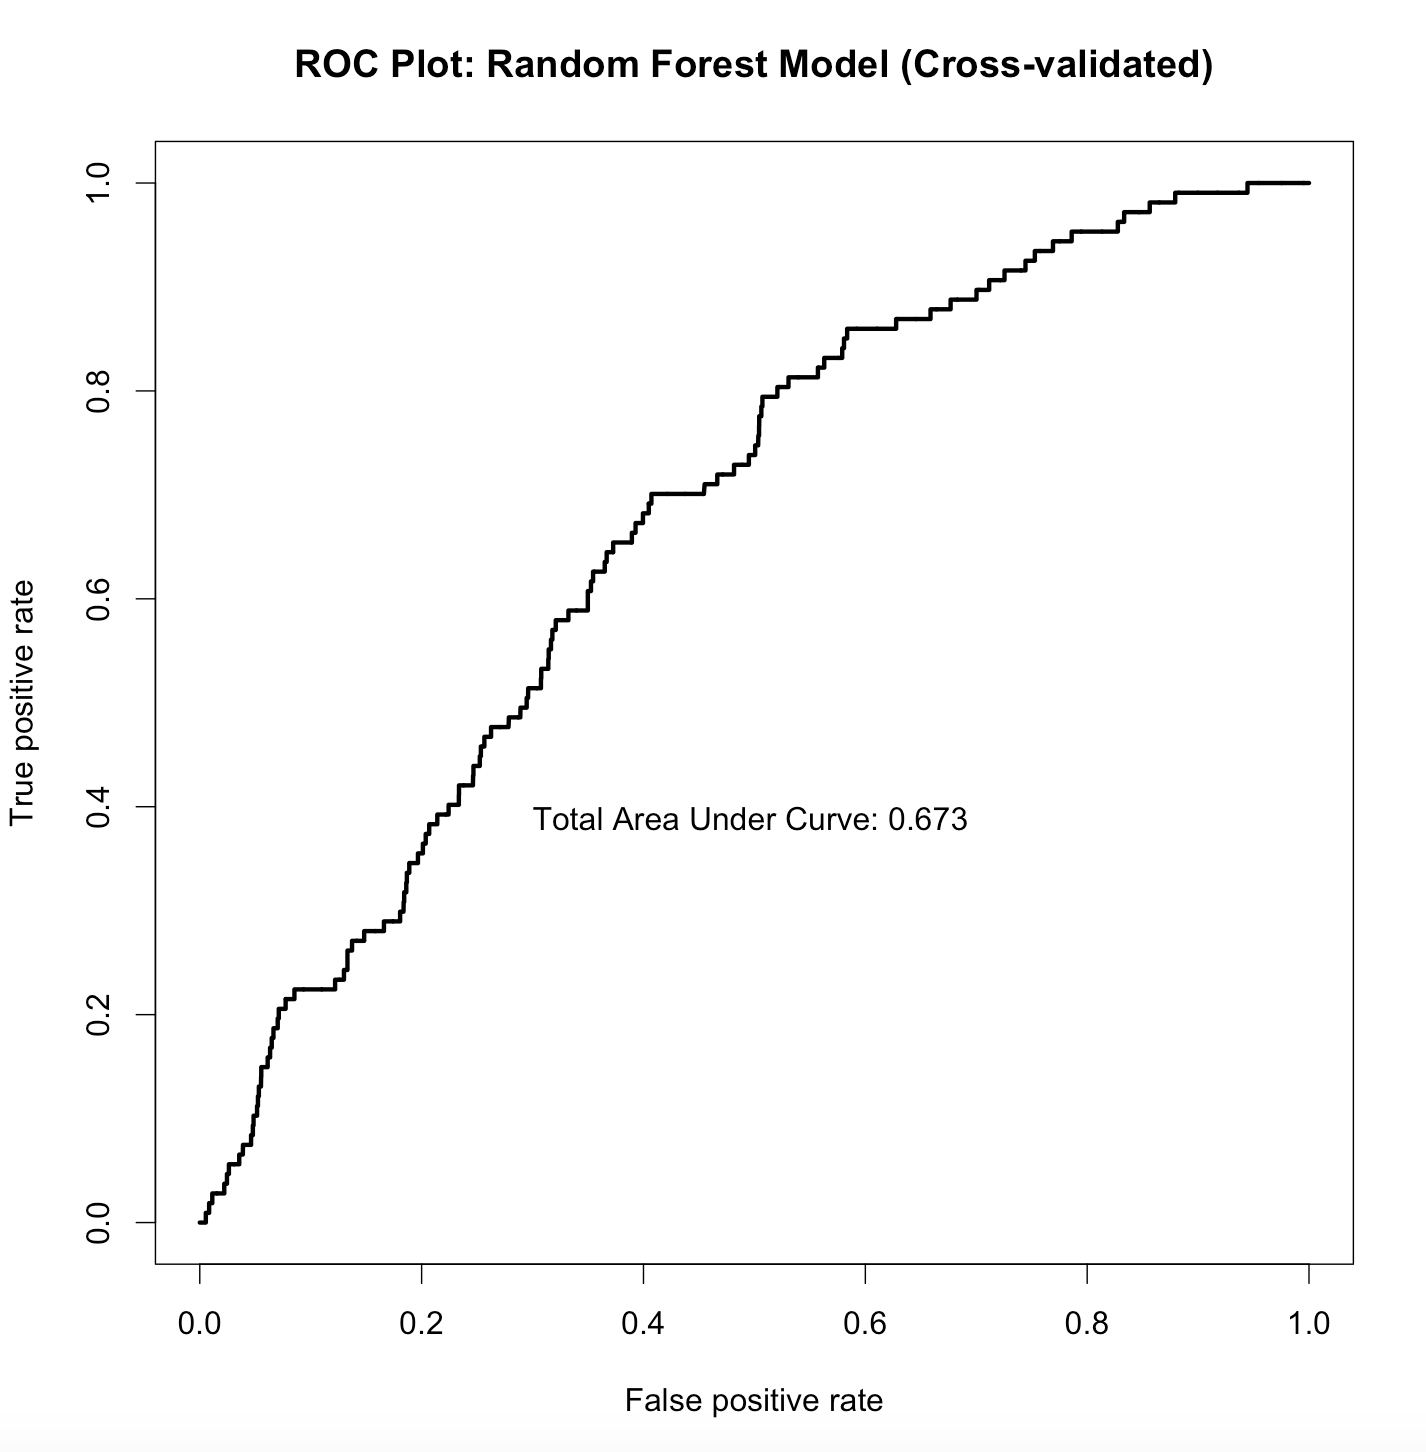
\includegraphics[width=0.5\linewidth]{rocrf.png}
    \caption{ROC Plot: Random Forest Model (Cross-validated)}
    \label{rocrf}
\end{figure}

However, the performance decreased from 0.741 to 0.673 (Figure \ref{rocrf}). Still, it generated useful information on the importance of the variables, suggesting population (\textit{lpop1}) and GDP (\textit{gdpenl}) to be the most important variables (Figure \ref{rf}). 

\begin{figure}[h!]
    \centering
    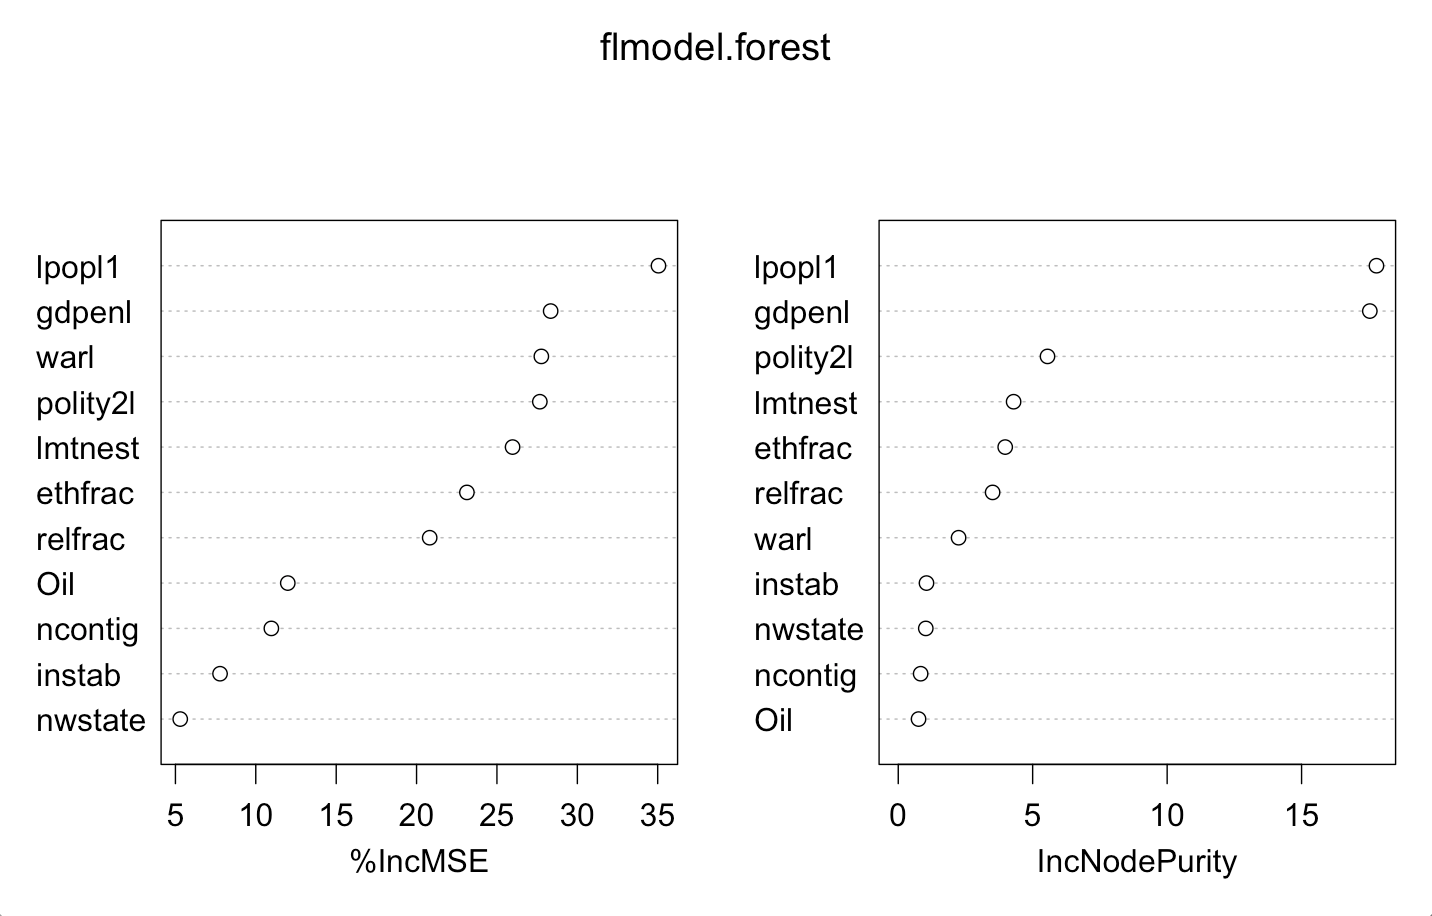
\includegraphics[width=\linewidth]{rf.png}
    \caption{Random Forest Importance Table}
    \label{rf}
\end{figure}

\section{Comparison}


\begin{table}[h!]
\centering
\caption{Performances of different models}
\label{my-label}
\begin{tabular}{|c|c|c|}
\hline
                                      & Predictive Power (AUC) & Out-of-sample Prediction Accuracy \\ \hline
Original Logistic Regression          & 0.761                               & N/A                                    \\ \hline
Logistic Regression (Cross Validated) & 0.741                               & 98.2\% (Threshold = 0.3)               \\ \hline
RPART (Cross Validated)               & 0.756                               & 98.3\%                                 \\ \hline
Random Forest (Cross Validated)       & 0.673                               & 97.8\% (Threshold = 0.3)               \\ \hline
\end{tabular}
\end{table}

As we can see in Table 2, although the original model has the highest predictive power, it has no use in predicting out-of-sample data. RPART Model successfully improves the Logistic Regression Model, while Random Forest performs worse.\footnote{\#probability}

One possible explanation is that, Fearon \& Laitin picked the predictors really well that the data points themselves were closer to a linear model. Therefore, the regression models including regression trees performed better than the random forest.  
\section{Discussions}
For current researchers researching on predictive models for various conflicts, Ward et al.'s conclusion still stands. Current models lack the predictive power and finding statistically significant predictors should not be the only focus. However, to add onto this point, researchers should never construct and analyze their models based on in-sample data. While acquiring new data is difficult, Cross Validation technics should always be performed to enable the models to have out-of-sample predictive powers. Out-of-sample heuristics including predictions should be the normal approach of all the research on conflicts.

For researchers who are working on discovering new predictors in civil conflicts, keep in mind that these technics are only for \textit{predictive} inferences, not \textit{causal} relationships. In other words, such models could only predict the chance of civil conflicts happening. It does not tell us these social factors (dependent variables) \textit{cause} civil conflicts. 

To really prevent a civil war from happening, researchers should focus on studying the causal relationship between different social factors and civil conflicts. Further research is needed before we could confidently say statements like "the low economic situation of this country is the main cause of its numerous civil conflicts."

\section{References}
Fearon, J. D., \& Laitin, D. D. (2003). Ethnicity, insurgency, and civil war. \textit{American political science review},\\ \indent 97(01), 75-90. \\
Ward, M. D., Greenhill, B. D., \& Bakke, K. M. (2010). The perils of policy by p-value: Predicting civil\\ \indent conflicts. \textit{Journal of Peace Research}, 47(4), 363-375. Chicago	

\section{Appendix}
Source code and \LaTeX\ documents available at: https://github.com/ZitongMao/CS112-Final

\begin{lstlisting}[language=R, caption=k-fold Cross Validation: Random Forest as an example]
library(plyr)
library(randomForest)
library(ROCR)

# loading data
load("~/CS112 Final/WGB Replication Files/Data/fl.three.RData")
data_test <- fl.three

set.seed(1)

# k-fold cross validation method

k = 5 # Folds

# sample from 1 to k, nrow times (the number of observations in the data_test)
data_test$id <- sample(1:k, nrow(data_test), replace = TRUE)
list <- 1:k

# prediction and testset data_test frames that we add to with each iteration over
# the folds
prediction.f <- data.frame()
prediction <- data.frame()
testsetCopy <- data.frame()

# creating a progress bar to visualize the CV process
progress.bar <- create_progress_bar("text")
progress.bar$init(k)

# loop for k times
for (i in 1:k) {
  # remove rows with id i from data_testframe to create training set
  # select rows with id i to create test set
  trainingset <- subset(data_test, id %in% list[-i]) #[-i] means except i
  testset <- subset(data_test, id %in% list[i])
  
  # run the random forest model
  flmodel.forest <- randomForest(onset ~ warl + gdpenl + 
                                   lpopl1 + lmtnest + ncontig + 
                                   Oil + nwstate + instab + polity2l
                                 + ethfrac + relfrac, data = trainingset, importance = TRUE)
  
  # getting predicted results
  temp <- as.data.frame(predict(flmodel.forest, testset))
  temp.f <- ifelse(temp > 0.3, 1, 0) # threshold
  
  # append this iteration's predictions to the end of the prediction data_test frame
  prediction <- rbind(prediction, temp)
  prediction.f <- rbind(prediction.f, temp.f)
  
  # append this iteration's test set to the test set copy data frame
  testsetCopy <- rbind(testsetCopy, as.data.frame(testset))
  
  progress.bar$step()
}

# add predictions and actual dependent variables values
result <- cbind(prediction.f, testsetCopy$onset)
names(result) <- c("Predicted", "Actual")
result$Difference <- result$Actual == result$Predicted

# use % correct classification 
table(result$Difference)
# % Accuracy
sum(result$Difference)/length(result$Difference)

# create ROC Plot
pred<- prediction(prediction, testsetCopy$onset)
perf<- performance(pred,"tpr","fpr")
plot(perf, main="ROC Plot: Random Forest Model (Cross-validated)", lwd=3)

# calculate the Area Under Curve (AUC)
auc <- performance(pred, measure = "auc")
auc <- auc@y.values[[1]]
auc

text(0.3,0.4,"Total Area Under Curve: 0.673",adj=c(0,1))

#show importance of variables in the random forest
varImpPlot (flmodel.forest)
\end{lstlisting}
\end{document}
